\documentclass{article}

% Language setting
% Replace `english' with e.g. `spanish' to change the document language
\usepackage[spanish]{babel}

% Set page size and margins
% Replace `letterpaper' with `a4paper' for UK/EU standard size
\usepackage[a4paper,top=2.5cm,bottom=2.5cm,left=3.5cm,right=3.5cm,marginparwidth=2.5cm]{geometry}

% Useful packages
\usepackage{amsmath}
\usepackage{graphicx}
\usepackage[gen]{eurosym}
\usepackage{siunitx}
%Podemos cambiar el color del Índice(negro), los enlaces están marcados en azul. 
\usepackage[colorlinks=true, linkcolor=black, urlcolor=blue]{hyperref}
\usepackage{fancybox}
\usepackage{listings}
\usepackage{subcaption}
%\lstset{
%    language=Matlab,
%    extendedchars=true
%}

\title{Diseño de Redes Inalámbricas en La Costera}
\author{Andé Yermak y Álvaro Hernández}
%\date{}

\begin{document}
\maketitle

%Aquí se generará nuestro Índice, podemos poner /newpage para tenerlo solo en la página
\tableofcontents
\newpage

\section{Introducción}

Se pretende dotar de acceso a internet a determinadas zonas de La Costera, Murcia. Una pedanía situada cerca de Alhama donde residen alrededor de 400 habitantes. La idea planteada será personalizar, según la necesidad, cada una de las zonas propuestas para su funcionamiento, y a su vez reducir al máximo el coste de instalación.

\begin{figure}[ht]
    \centering
    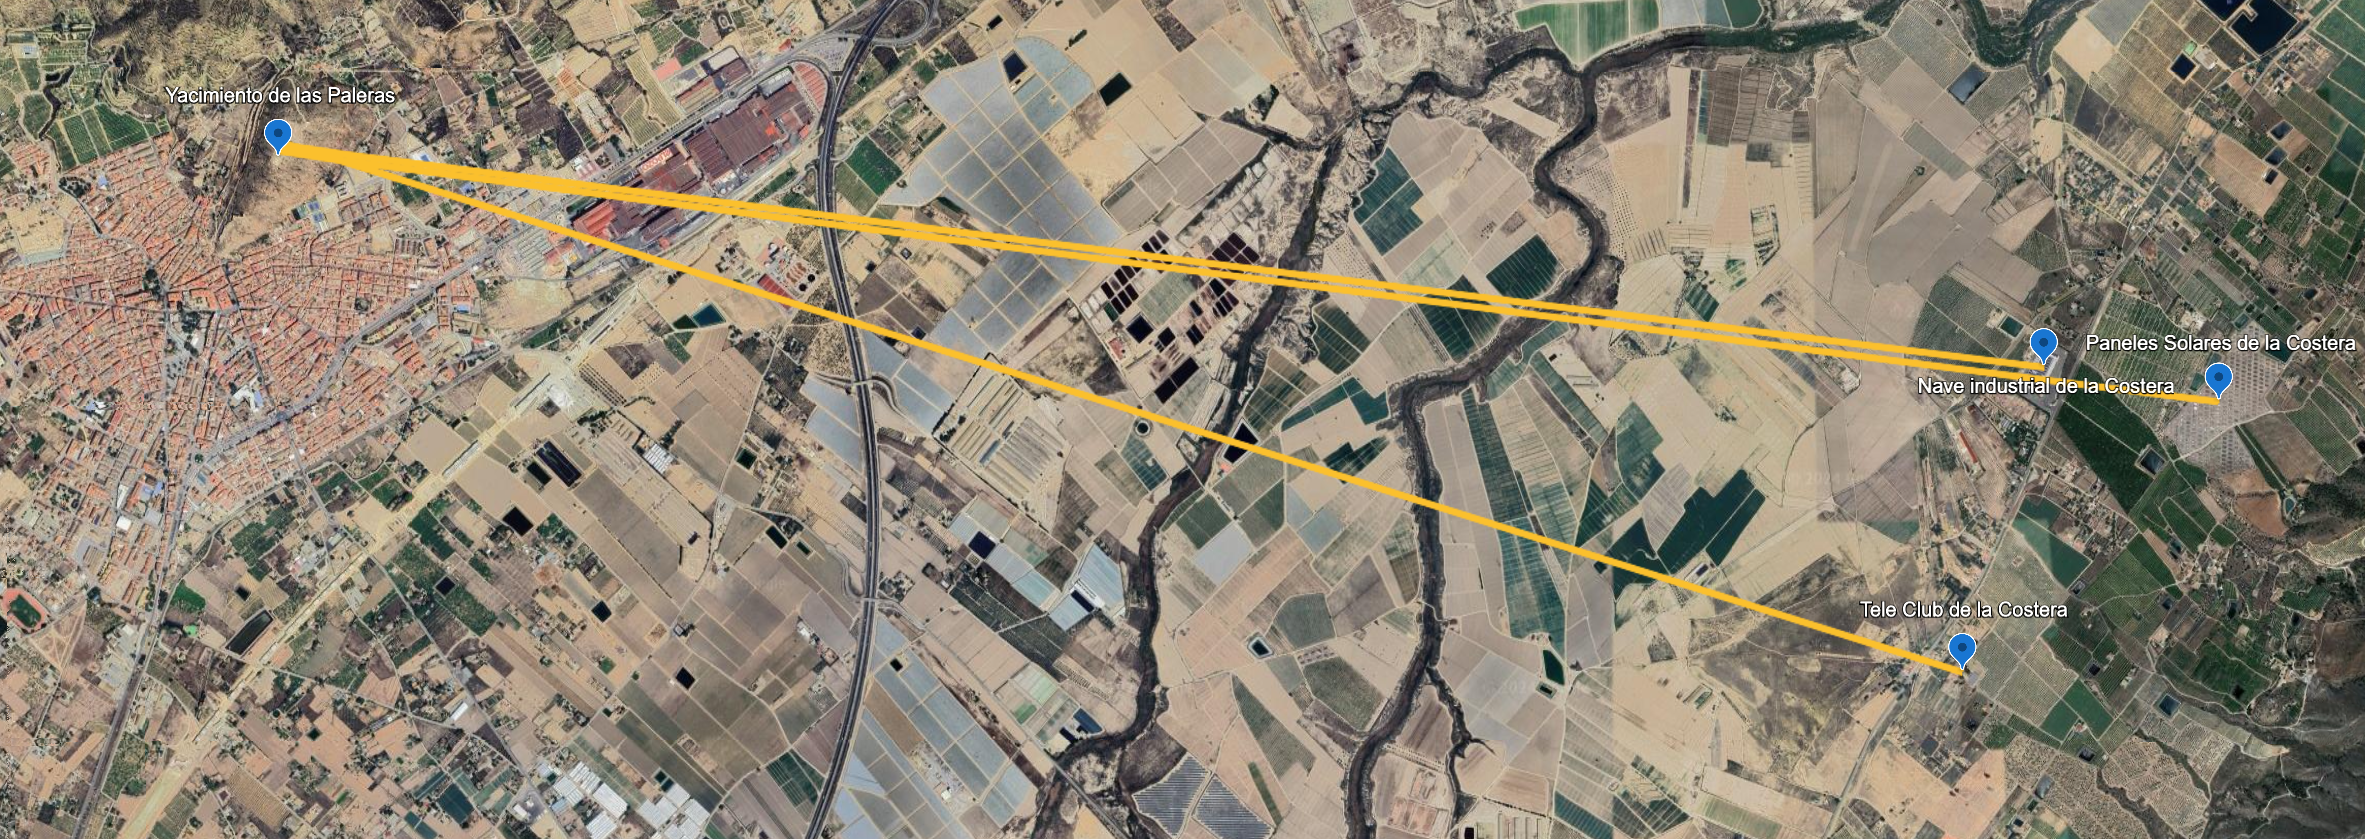
\includegraphics[width=0.8
    \linewidth]{src/earthpoints.png}
    \caption{\label{fig:earthpoints} Mapa de los puntos de radio enlace.}
\end{figure}

\quad

Al ser un servicio propuesto por el ayuntamiento, se usarán bandas de frecuencia de la red troncal, es decir, de $5GHz$ y de $2.4GHz$, donde no será necesario cierta cantidad de trámites para usarlas a comparación de otras personalizadas, además de ser gratis el añadido de radioenlaces. Por otro lado, se limitarán ciertos parámetros como la potencia de transmisión.

\quad

Las coordenadas de las distintas secciones serán:

\quad

\textbf{TeleClub}:
\begin{itemize}

    \item Latitud: 37.8390744
    \item Longitud: -1.3648323

\end{itemize}

\quad

\textbf{La nave}:
\begin{itemize}

    \item Latitud: 37.8390744
    \item Longitud: -1.3648323

\end{itemize}

\quad

\textbf{Paneles}:
\begin{itemize}

    \item Latitud: 37.8390744
    \item Longitud: -1.3648323

\end{itemize}


\subsection{Planteamiento de TeleClub}

El teleclub es un centro social que necesita de internet tanto \textbf{indoor} como \textbf{outdoor}. De puertas para dentro estará la biblioteca, lugar donde la conexión es de suma importancia para tareas como descarga de ebooks o registros en su web de usuarios. En el exterior del teleclub, se dotará de internet básico para el ocio que puedan tener los visitantes y residentes, se tiene en cuenta que el exterior tendrá un mayor número de usuarios.

\quad

\begin{figure}[ht]
    \centering
    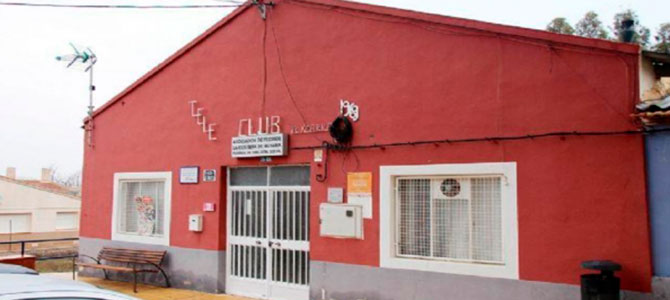
\includegraphics[width=0.5\linewidth]{src/teleclub.jpg}
    \caption{\label{fig:teleclub} Fachada del TeleClub.}
\end{figure}


Según la población de \textbf{La Costera}, que es de 343 habitantes, (Actualizado febrero 2023), se puede considerar que el tráfico de TeleClub no superará el 20\% de la población total. Ésto es de aproximadamente 75 usuarios. Se añadirá un margen debido al turismo de 25 usuarios, por lo que el máximo tráfico cursado será de \textbf{100 usuarios}.

\quad

Para calcular el \textbf{throughput} que consumirá nuestra sección del TeleClub, se planteará el concepto de \textbf{usuario típico}, y se multiplicará la velocidad máxima por la cantidad de éstos. Será aquél que utiliza el correo, navega por Internet y ocasionalmente transmite/recibe ficheros de gran tamaño. A día de hoy, es necesario tener una buena latencia y velocidad, por lo que se usará la velocidad máxima limitada que normalmente se permite en conexiones \textbf{red-usuario} típicas, que es de 256kbps.

    $$100u \cdot 256kbps = 25600kbps = 25Mbps $$

El throughput para esta zona será de \textbf{25Mbps}.

\subsection{Planteamiento de la Nave}

En la Nave habrá un máximo de 30 usuarios. Según la guía del trabajo, habrá, entre servidores y tráfico de usuarios una tasa de bits de unos \textbf{10Mbps} como máximo, por lo que definirá el throughput de esta sección. 

\quad

Puesto que no se conoce qué zonas serán de mayor importancia o no requieran de acceso a internet, habrá 4 AP repartidos de manera uniforme, donde se usará la infraestructura con \textbf{VAPs} para alejar dos redes inalámbricas distintas: para trabajadores y empleados.

\begin{figure}[ht]
    \centering
    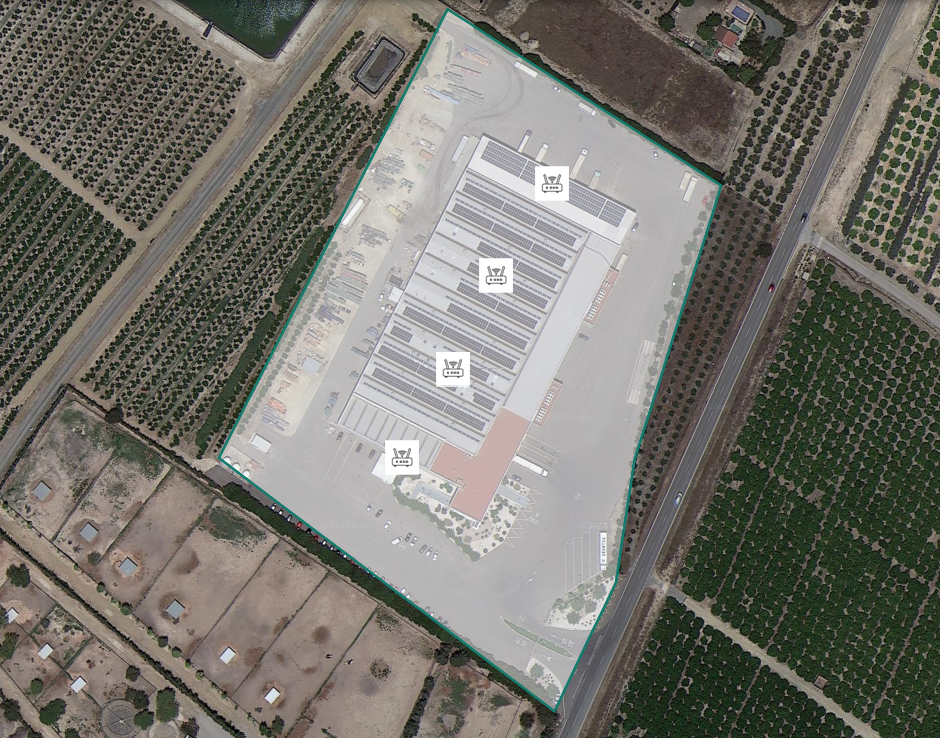
\includegraphics[width=0.65\linewidth]{src/lanave.png}
    \caption{\label{fig:lanave} Reparto de APs en la nave.}
\end{figure}

\newpage

\subsection{Planteamiento de Paneles}

El recinto de paneles, se requerirá una cierta cantidad de cámaras ya que es necesario una vigilancia para mayor seguridad de la zona, debido a posibles robos. En lugar de repartir todas las cámaras por el área, se colocarán cámaras repartidas por todo el perímetro de la zona, de tal modo que no sería necesario vigilar el interior, pues estaría grabada la entrada al recinto de cualquier persona.

\quad

Al ser 30 metros el radio de cada cámara, habrá entre cada una 60 metros de distancia. Se reparten uniformemente por todo el perímetro, según las medidas de \textbf{Google Earth}. También habrán APs repartidos por toda la zona para dotar la conexión necesaria a las cámaras. 
\begin{figure}[ht]
    \centering
    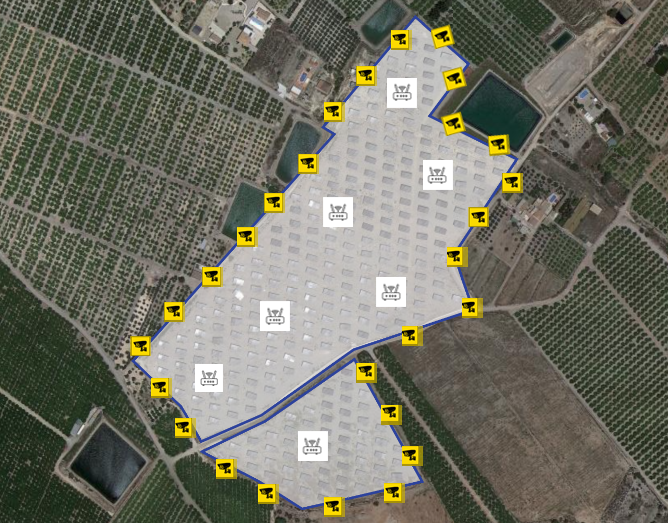
\includegraphics[width=0.4\linewidth]{src/camaras.png}
    \caption{\label{fig:camarasnave} Reparto de las cámaras y access points.}
\end{figure}

Se considerará el tráfico de cada cámara de \textbf{1Mbps}, por lo que, tras el reparto de cámaras por distancias, al haber un total de \textbf{28 unidades}, el throughput de esta sección será: 

$$28u \cdot 1Mbps = 28Mbps$$

\section{Materiales elegidos}

\subsection{Materiales comunes}
Los switches se eligirán unos económicos de una marca confiable, puesto que el uso que se hará en un pueblo de pocos habitantes será mucho menor a otros que requieren de tecnología más sofisticada. Éstos switches suelen tener vida útil limitada, pero es con respecto a la garantía, no significa que su uso esté limitado a cierto tiempo:

\quad

Para los switches que requieran 8 puertos o menos se usará el \textbf{Switch TL-SG108E Easy Smart de 8 puertos Gigabit}, de la marca TP-link. Se trata de un switch no gestionado y económico, diseñado para pequeñas y medianas empresas que requieren de redes con gestión simple. Para optimizar el tráfico en su red de negocios, el switch ofrece QoS basado en puerto y en etiquetas para mantener el tráfico sensible a la latencia sin problemas y sin fluctuaciones. Además, el gasto energético no será elevado, puesto que el TL-SG108E puede ahorrar hasta un 80\% del consumo de energía, lo cual es una solución ecológica para su red de negocios. 

Para la nave, donde hará falta uno de más puertos, se usará el \textbf{TP-Link TL-SF1016DS de 16 puertos.} Ya que el modelo anterior no tiene opción de más puertos, este sería su equivalente. 
\newpage

\begin{figure}[h]
	\centering
	\begin{subfigure}{0.3\textwidth}
		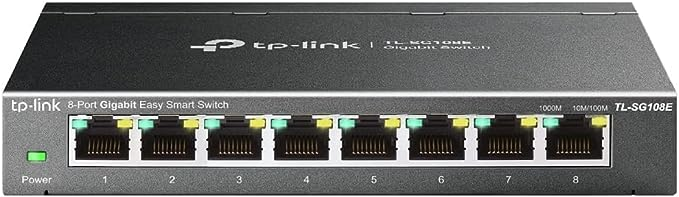
\includegraphics[width=\linewidth]{src/switch 8.jpg}
		\caption{Switch de 8 Puertos}
		\label{fig:switch8}
	\end{subfigure}%
	\begin{subfigure}{0.3\textwidth}
		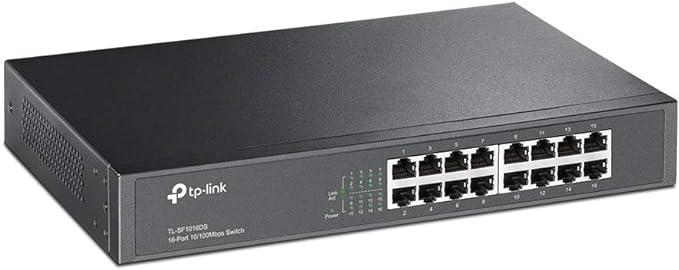
\includegraphics[width=\linewidth]{src/switch 16.jpg}
		\caption{Switch de 16 Puertos}
		\label{fig:switch16}
	\end{subfigure}
	\caption{}
	\label{fig:switches}
\end{figure}

Los access points serán de la marca \textbf{Ubiquiti}, al igual que las antenas usadas. En este caso, el \textbf{Ubiquiti Networks UAP-AC-LR}. Según su \href{https://dl.ubnt.com/datasheets/unifi/UniFi_AC_APs_DS.pdf}{Datasheet}, tiene soporte para VLANs, protocolos de privacidad y seguridad como \textbf{WPA2}, y compatibilidad con las antenas Ubiquiti elegidas.

\quad

Se usará una estación base Ubiquiti Rocket R2AC-PRISM al ser la que mejor cumple las necesidades con un coste reducido, al igual que una compatibilidad con las antenas \textbf{Ubiquiti}. De tal modo que se podrá crear un ecosistema de la misma marca en distintos puntos con compatibilidad y fácil asistencia. Según su \href{https://dl.ubnt.com/datasheets/RocketAC/Rocket_R2AC_DS.pdf}{Datasheet}, consigue un SNR elevado, y trabaja solo en frecuencias de $2.4GHz$, de este modo se consigue una reducción del precio al no usarse en ningún momento bandas de frecuencia de $5GHz$.

\begin{figure}[ht]
	\centering
	\begin{subfigure}{0.35\textwidth}
		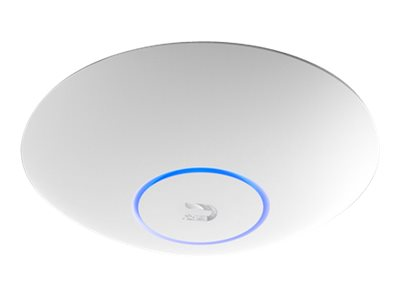
\includegraphics[width=\linewidth]{src/ap.jpg}
		\caption{Access Point Ubiquiti}
		\label{fig:ap}
	\end{subfigure}%
	\begin{subfigure}{0.25\textwidth}
		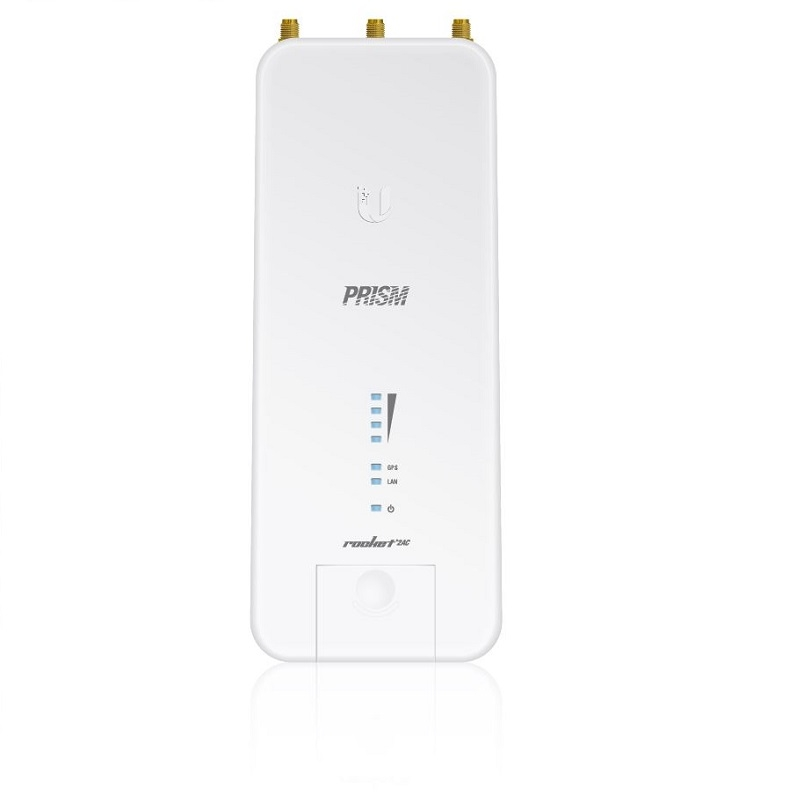
\includegraphics[width=\linewidth]{src/estacion base.jpeg}
		\caption{Estación Base}
		\label{fig:estacionbase}
	\end{subfigure}
	\caption{}
	\label{fig:accesspoint}
\end{figure}
\subsection{Radioenlaces}

Se ha proporcionado en el aula virtual un \href{http://www.microcom.com.ar/fotos/ficha7097LBE-M5-23.compressed.pdf}{Datasheet} donde aprovecharemos para elegir el material que más se adapte a nuestros planteamientos. 

\quad

Se usará de antena transmisora el Ubiquiti LBE-5AC-16-120, ya que al ser omnidireccional permite transmitir en distintas direcciones. Dicha antena se situará en Alhama, específicamente en el Yacimiento de las Paleras, por tener mayor elevación respecto al resto de la zona para una transmision mejor. Junto a esta antena, se conectará la estación base Rocket Prism R2AC.

\quad

En las otras tres ubicaciones, situadas en la \textbf{Nave}, \textbf{TeleClub}, y los \textbf{paneles}, se usarán antenas unidireccionales pusto que su única conexión será con la antena transmisora. En el \textbf{Datasheet proporcionado}, la antena que cumple con los requisitos es la Ubiquiti LBE-5AC-23.

En el \textbf{TeleClub}, se recibe la señal principal en la antena LBE-5AC-23, y se repartirá la conexión mediante un switch a dos Access Points: que servirán para \textbf{Indoor} y \textbf{Outdoor}. No hay material adicional.

\quad

En la \textbf{nave}, se usarán 4 APs repartidos uniformemente en la zona, además de la antena LBE-5AC-23, tampoco habrá material adicional.

\quad

En los \textbf{paneles}, además de los APs y la antena, es necesario elegir las cámaras usadas. Se ha optado por un modelo de \textbf{Anksono}, ya que cumple con el requisito de ser económica por la cantidad que hay que añadir, y el rango de vigilancia es similar a otras de mayor precio.

\section{Presupuesto}

Se sumarán al presupuesto las 3 torretas que se usan para que los radioenlaces tengan una altura correcta, con las antenas ya elegidas, y así evitar obstáculos y atenuación. En este caso, se elegirá una torreta de \textbf{5 metros} en Alhama, y para las demás serán de \textbf{1.65 metros} debido a que el tejado ya está alto y se suma a las torretas. La tabla de presupuestos será:

\begin{table}[ht]
    \centering
    \begin{tabular}{|c|c|c|c|}
        \hline
        Material & Cantidad & Precio & Suma \\
        \hline
        Switch TL-SG108E & 2 & $31.99\euro{}$ & $63.98\euro{}$ \\
        Switch TL-SF1016DS & 1 & $59.69\euro{}$ & $119.38\euro{}$ \\
        Ubiquiti LBE-5AC-16-120  & 1 & $102.58\euro{}$ & $102.58\euro{}$ \\
        Ubiquiti LBE-5AC-23& 2 & $73.89\euro{}$ & $147.78\euro{}$ \\
        E. Base R2AC-PRISM & 1 & $207.50\euro{}$ & $207.50\euro{}$ \\
        
        Cámaras Anksono& 28 & $29.99\euro{}$ & $839.72\euro{}$ \\
        Ubiquiti UAP-AC-LR & 13 & $89.00\euro{}$ & $1157.00\euro{}$ \\
        
        Torreta de 5 metros& 1 & $336.32\euro{}$ & $336.32\euro{}$ \\
        Mástiles de 1.65 metros & 3 & $53.32\euro{}$ & $159.96\euro{}$ \\
        \hline
        Total &  &  & $3134.22\euro{}$ \\
        \hline
    \end{tabular}
    \caption{Tabla del presupuesto total }
    \label{tab:presupuestos}
\end{table}



\section{Normativa PIRE}

La banda de frecuencias 2400-2483,5 MHz, designada en el Reglamento de
Radiocomunicaciones para aplicaciones industriales, científicas y médicas (ICM),
podrá ser utilizada también para los siguientes usos de radiocomunicaciones bajo la
consideración de uso común:

\begin{itemize}

    \item Sistemas de transmisión de datos de banda ancha y de acceso inalámbrico
    a redes de comunicaciones electrónicas incluyendo redes de área local.

\end{itemize}

    Estos dispositivos pueden funcionar con una potencia isotrópica radiada equivalente
    (p.i.r.e.) máxima de 100 mW conforme a la Decisión de Ejecución (UE) 2017/1483
    Notas UN CNAF 2017 Página 37
    de la Comisión por la que se modifica la Decisión 2006/771/CE, sobre la
    armonización del espectro radioeléctrico para su uso por dispositivos de corto
    alcance y a la Recomendación CEPT ERC/REC 70-03, anexo 3.
    Además, la densidad de potencia (p.i.r.e.) será de 100 mW/100 kHz con modulación
    por salto de frecuencia y de 10 mW/MHz con otros tipos de modulación. En ambos
    casos, se deberán utilizar técnicas de acceso y mitigación de interferencias con
    rendimiento al menos equivalente a las técnicas descritas en las normas
    armonizadas según la Directiva 2014/53/UE.
    En cuanto a las características técnicas de estos equipos, la norma técnica de
    referencia es el estándar ETSI EN 300 328 en su versión actualizada.

\begin{itemize}
    \item Dispositivos genéricos de baja potencia en recintos cerrados y exteriores
    de corto alcance, incluyendo aplicaciones de video.
\end{itemize}
    La potencia isotrópica radiada equivalente máxima será 10 mW, conforme a la
    Decisión de Ejecución (UE) 2017/1483 de la Comisión por la que se modifica la
    Decisión 2006/771/CE, sobre la armonización del espectro radioeléctrico para su uso
    por dispositivos de corto alcance y a la Recomendación CEPT ERC/REC 70-03,
    Anexo 1, siendo la norma técnica de referencia el estándar ETSI EN 300 440. 


\section{Radioenlaces}

\subsection{Parámetros y modulación de las antenas}

Teniendo en cuanta la tabla de mcsindex habrá que calcular los throughput de cada sección para asegurar que el sistema soportará el momento de mayor tráfico, que decidirá la modulación usada. 

Siendo el throughput total:

$$25Mbps + 10Mbps + 28Mbps = 63Mbps$$

Por lo que para elegir la modulación usada, se tendrá en cuenta que supere el throughput necesario. En este caso, al ser MIMO la antena y trabajar en $2.4Ghz$, la modulación adecuada será:

\begin{figure}[ht]
    \centering
    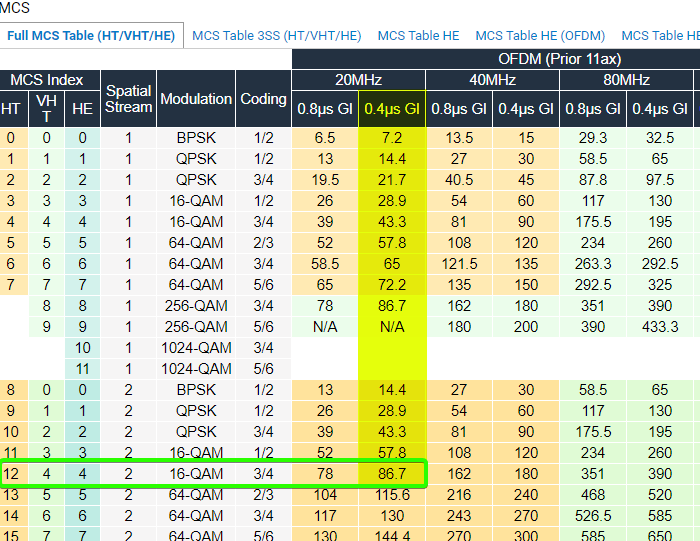
\includegraphics[width=0.8
    \linewidth]{src/mcsindex.png}
    \caption{\label{fig:mcsindex} Modulación elegida.}
\end{figure}

Se elige 16-QAM 3/4. Viendo el \textbf{datasheet}, la antena receptora tendrá una sensibilidad de -86dBm y margen de 2, por lo que se elige la peor posibilidad, -84dBm.

\subsection{RadioMobile}

\subsection{Configuración y parámetros}

A continuación, se mostrarán capturas del programa RadioMobile, donde se han configurado todos los parámetros necesarios para hacer una conexión correcta entre todos los enlaces planteados. 

\quad

Se han tenido en cuenta todos los parámetros, datos y regulaciones mencionadas anteriormente:

\begin{figure}[ht]
    \centering
    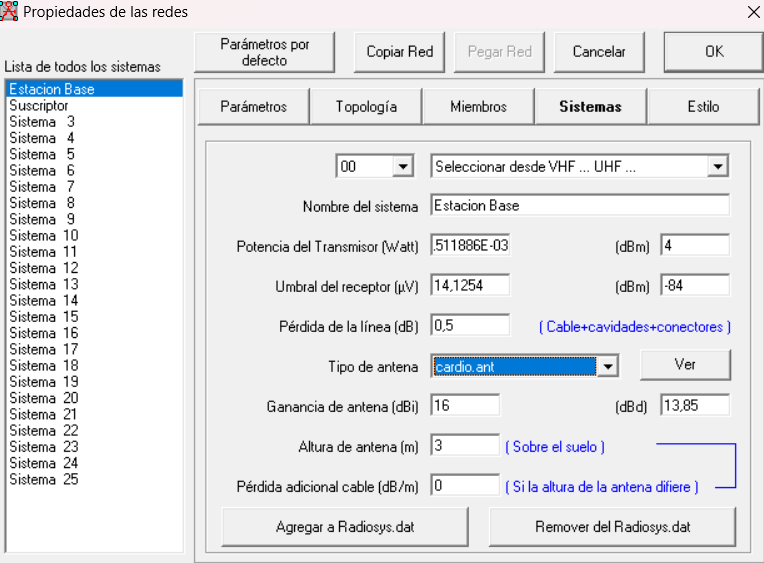
\includegraphics[width=0.7\linewidth]{src/estacionbase.png}
    \caption{\label{fig:ebaseconfig} Configuración de la estación base.}
\end{figure}

\begin{figure}[ht]
    \centering
    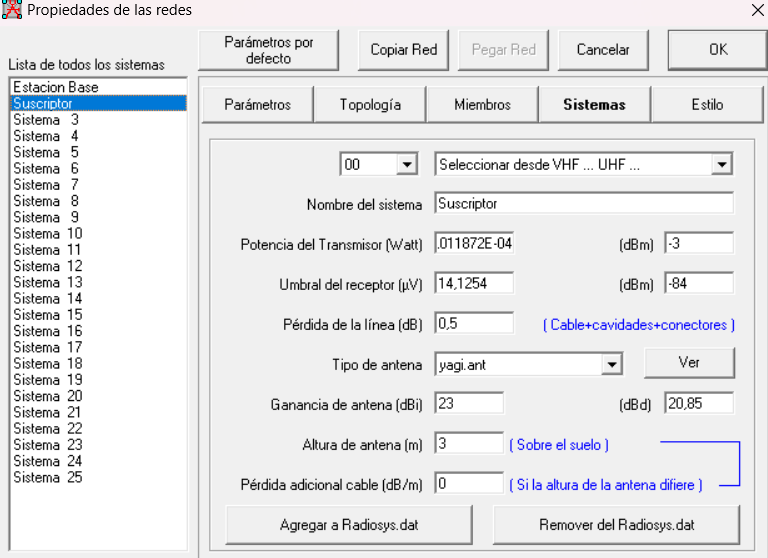
\includegraphics[width=0.7\linewidth]{src/suscriptor.png}
    \caption{\label{fig:suscripconfig} Configuración del suscriptor.}
\end{figure}

\newpage

\subsection{Visualización de radioenlaces}

Los radioenlaces serán:

\begin{figure}[ht]
    \centering
    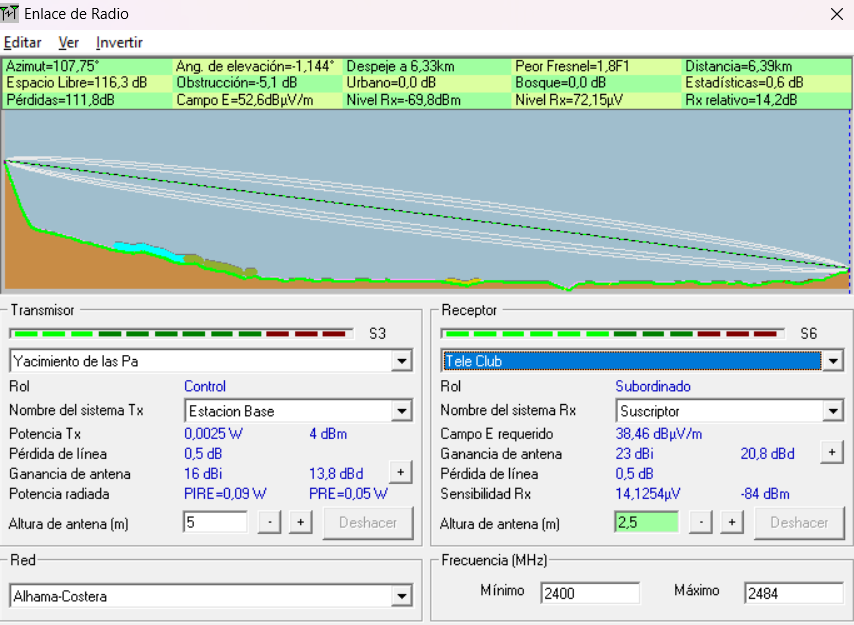
\includegraphics[width=0.8\linewidth]{src/EstacionBase-TeleClub.png}
    \caption{\label{fig:ebaseteleclub} Estación base a teleclub.}
\end{figure}

\newpage

\begin{figure}[ht]
    \centering
    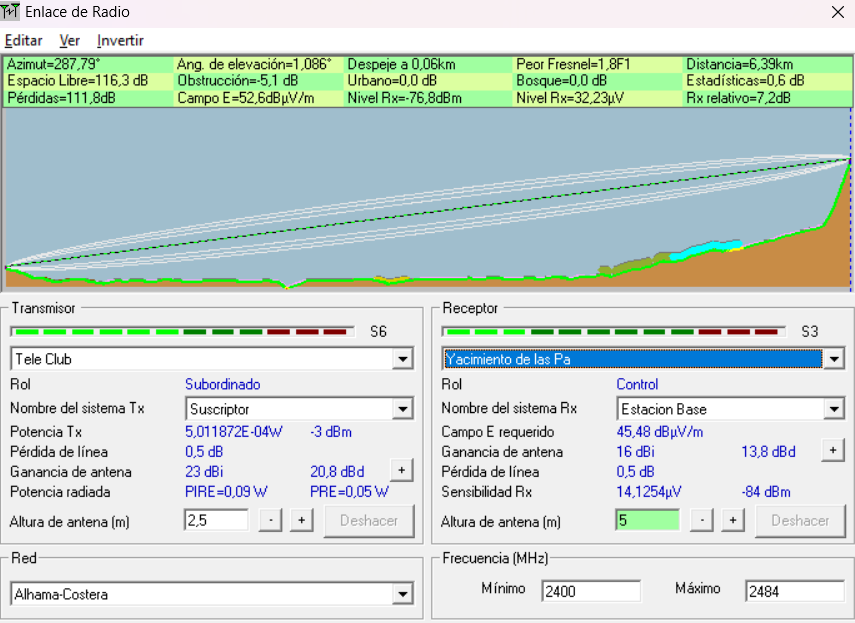
\includegraphics[width=0.8\linewidth]{src/TeleClub-EstacionBase.png}
    \caption{\label{fig:teleclubebase} Teleclub a estación base.}
\end{figure}

\begin{figure}[ht]
    \centering
    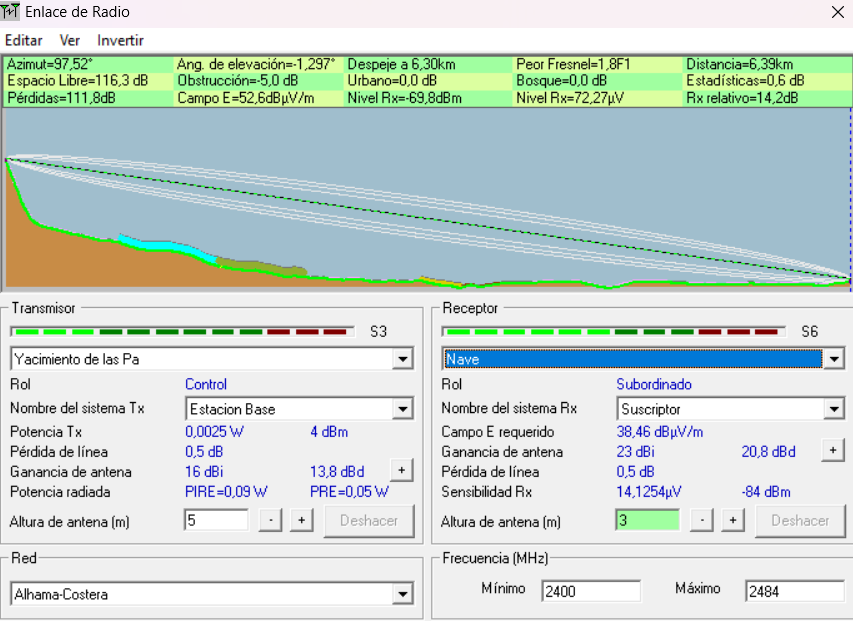
\includegraphics[width=0.8\linewidth]{src/EstacionBase-Nave.png}
    \caption{\label{fig:ebasenave} Estación base a nave.}
\end{figure}
\newpage

\begin{figure}[ht]
    \centering
    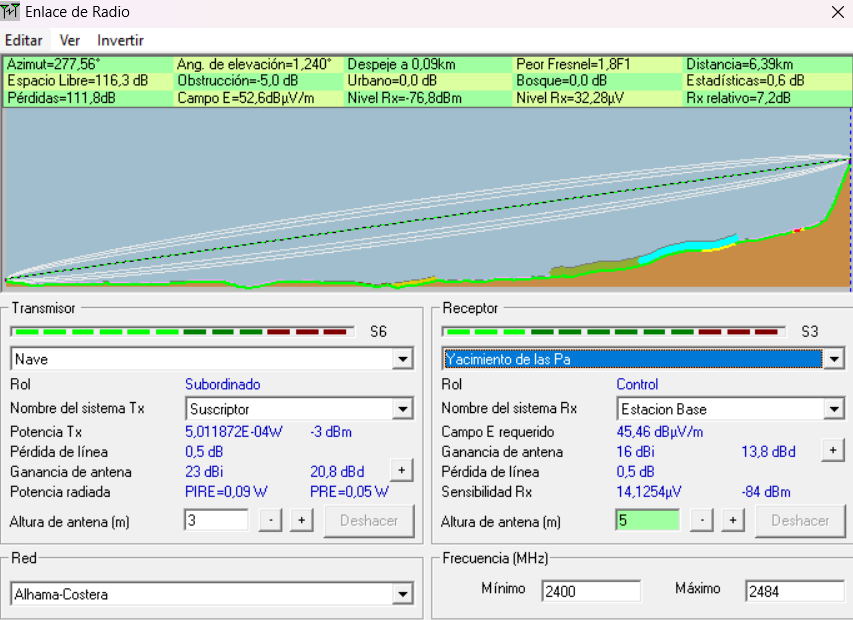
\includegraphics[width=0.8\linewidth]{src/Nave-EstacionBase.png}
    \caption{\label{fig:naveebase} Nave a estación base.}
\end{figure}

\begin{figure}[ht]
    \centering
    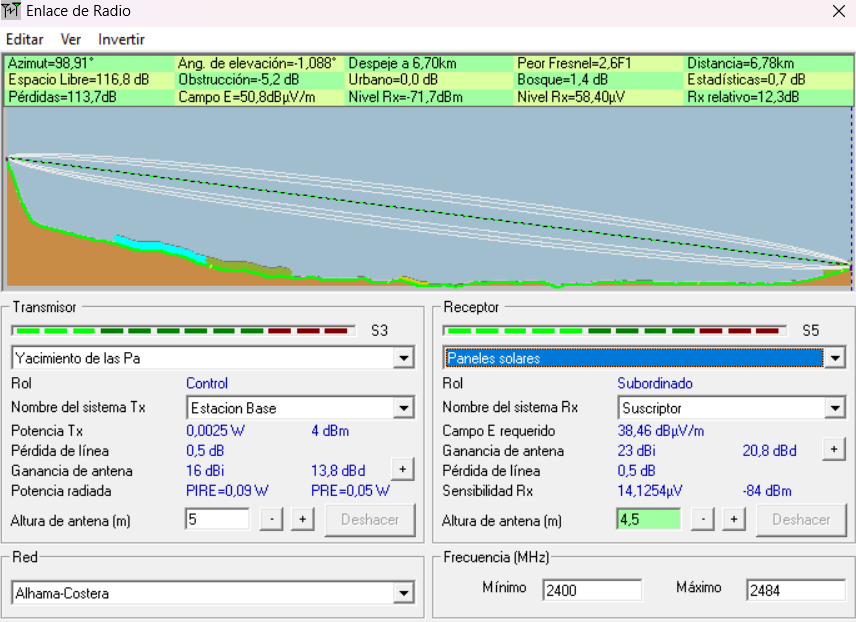
\includegraphics[width=0.8\linewidth]{src/EstacionBase-Paneles.png}
    \caption{\label{fig:ebasepaneles} Estación base a paneles.}
\end{figure}

\newpage
\begin{figure}[ht]
    \centering
    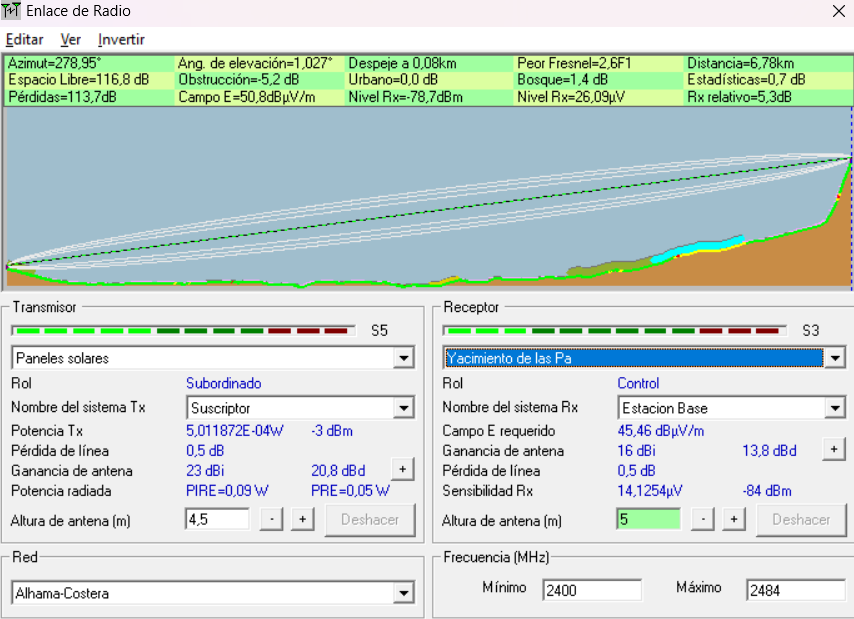
\includegraphics[width=0.8\linewidth]{src/Paneles-EstacionBase.png}
    \caption{\label{fig:panelesebase} Paneles a estación base.}
\end{figure}

Se tendrá en cuenta el direccionamiento de las antenas para la correcta transmisión, en caso contrario, el enlace daría error en el programa. De igual manera que la altura, contando la torreta y el mástil, también es necesaria para marcar, ya que el balance depende de ello y los obstáculos que haya.

\quad

Finalmente, todas las configuraciones de los materiales con los datos previamente establecidos, dará lugar a una correcta conexión entre los tres enlaces:
\newpage
\begin{figure}[ht]
    \centering
    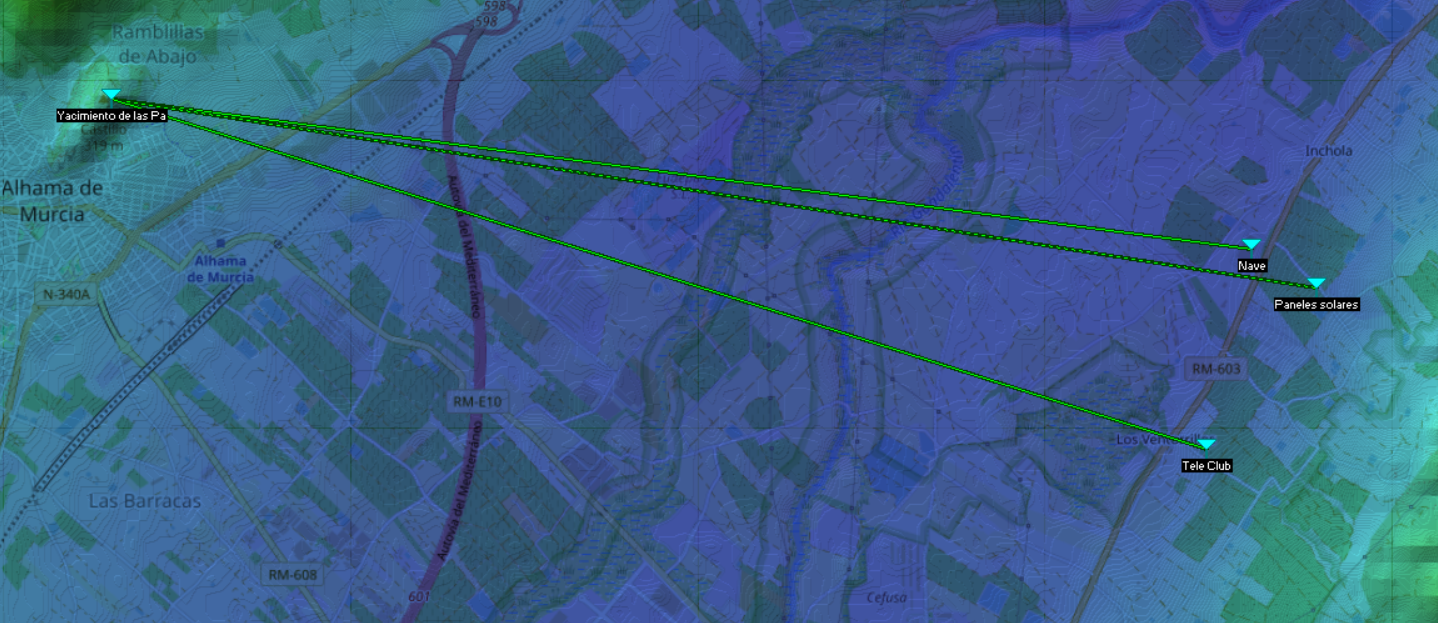
\includegraphics[width=1\linewidth]{src/mapa radio.png}
    \caption{\label{fig:maparadio} Mapa del resultado de los radioenlaces.}
\end{figure}

\section{Diseño de la Red}


\begin{figure}[ht]
    \centering
    \includegraphics[width=1\linewidth]{src/diseñored.jpg}
    \caption{\label{fig:diseñored} Diseño de la red.}
\end{figure}

El diseño del proyecto consta principalmente de 3 radio enlaces formados entre:

\begin{itemize}
    \item $\text{Alhama} \rightarrow \text{La Nave}$
    \item $\text{Alhama} \rightarrow \text{Paneles solares}$
    \item $\text{Alhama} \rightarrow \text{TeleClub}$
\end{itemize}

En Alhama se situarán todos los sistemas que gestionarán la red, que serán los \textbf{servidores DHCP} que proporcionan la dirección IP a cada zona, el\textbf{ portal cautivo} el cual da acceso a internet a todos los residentes que entren desde Teleclub a Internet, los \textbf{servidores radius}; uno para los empleados de red y trabajadores de la nave que empleará el protocolo WPA2-ENTERPRISE, y otro para las cámaras que podría emplear también WPA2-ENTERPRISE, y un \textbf{router} que de acceso a internet.

\quad

Dicha antena transmisora está configurada según la normativa vista en los apartados anteriores (100 mW max. PIRE): 

$$P_{TX} = 4dBm \quad \text{Sensibilidad}=-84dB \quad G_i=16 dBi$$

Las tres antenas receptoras estarán configuradas por igual para que se pueda aplicar la misma técnica de modulación: 

$$P_{TX} = -3dBm \quad \text{Sensibilidad}=-84dB \quad G_i=23 dBi$$

En cada zona objetivo se verá que hay VAP que diferencia entre usuarios corrientes respecto a los usuarios especiales que son los empleados de red y administraciones públicas (que será igual dicha IP en cada zona: 192.168.0.0 es la red asignada por el DHCP y habrán un total de 5 usuarios por zona)

\quad

En la nave, se conectará un switch que permita enlazar todos los usuarios conectados a los AP (por simplificación se ha mostrado 1 simulando los 4), los trabajadores de la nave tienen asignadas por el DHCP la red 192.168.3.0 (con una suma de 25 trabajadores)
En la zona de los paneles solares habrán conectadas cámaras a las distintas VAPs repartidas por toda la zona, las IPs asignadas serán 192.168.2.0 (con un total de 28 usuarios=cámaras). Dichas cámaras serán monitorizadas desde Alhama, es por eso que posee una conexión directa desde ahí.

\quad

En TeleClub habrán ahora 2 APs con 2 VAPs, diferenciando indoor y outoor y que tanto como empleados como los residentes (y turistas) tengan acceso a la red en cualquier parte de la zona. La red asignadas para los residentes es 192.168.1.0 (95 usuarios).

\newpage

\section{Enlaces utilizados}

\quad

\quad

\href{https://www.generadordeprecios.info/obra_nueva/Instalaciones/Audiovisuales/Red_de_cables_coaxiales/Mastil_para_fijacion_de_antenas.html#gsc.tab=0}{Calculador de precio mástil}

\quad

\href{https://generadordeprecios.info/obra_nueva/calculaprecio.asp?Valor=0|0_0_0_0|1|IAA032|iaa_032:_0_0_0_0_0_1_0#gsc.tab=0}{Calculador de Precio torreta}

\quad

\href{https://www.amazon.es/TP-Link-TL-SF1016DS-escritorio-puertos-100Mbps/dp/B0054TXRVQ/}{TP-Link TL-SF1016DS}

\quad

\href{https://www.amazon.es/TP-Link-TL-SG108E-configuraci%C3%B3n-administrada-priorizaci%C3%B3n/dp/B00JKB63D8}{TP-Link TL-SG108E}

\quad

\href{https://www.amazon.es/Ubiquiti-UAP-AC-LR-Punto-Acceso-inal%C3%A1mbrico/dp/B016K5A06C?th=1}{Ubiquiti UAP-AC-LR Punto de Acceso}

\quad

\href{https://www.amazon.es/dp/B09K7HVKLT/ref=tsm_1_fb_lk}{Cámara}

\quad

\href{https://mcsindex.com/}{MCS Index}

\quad

\href{https://www.ve2dbe.com/english1.html}{RadioMobile web}

\quad


\href{https://earth.google.com/web/}{Google Earth}

\quad

\href{http://labit501.upct.es:8080/}{NetEval}

\quad

\href{https://avancedigital.mineco.gob.es/espectro/CNAF/notas-UN-2017.pdf}{Notas UN del estado}

\quad

\href{https://maker-store.es/home-office/wireless-lan/wireless-lan-antennen/3748/ubiquiti-r2ac-prism-rocket-basestation}{Ubiquiti R2AC Prism Rocket Basestation}

\quad

\href{https://www.pccomponentes.com/ubiquiti-networks-litebeam-ac-gen2-airmax-ac-5ghz?srsltid=AfmBOorsXOMoawlF2P6S67Bx6O224uWPzhzismqEu5VPiAxKXXhdxbW32vw}{Ubiquiti Networks LiteBeam AC Gen2 AirMAX AC 5GHz}

\quad

\href{https://www.amazon.es/UBIQUITI-Networks-LBE-5AC-16-120-Repetidor-5-15-5-875/dp/B019M0KK44}{UBIQUITI Networks LBE-5AC-16-120}

\end{document}